\chapter{Evaluation}

In this section, we first categorize \ematching patterns into three categories. Next, we evaluate our prototype of relational \ematching with two preliminary experiments, choosing patterns from each of the categories, and discussed our progress on evaluating full-system benchmarks. More experiment will be presented in the forthcoming paper.


To investigate the kinds of conjunctive queries an \ematching pattern would generate and its performance implication on the join algorithms, we categorize the \ematching patterns into three categories according to the kinds of conjunctive queries they generate:
\begin{enumerate}
    \item Linear patterns: this is the simplest form of patterns, where no variables occur more than once in the pattern. Examples of this category include $f(\alpha, \beta)$ and $f(g(\alpha),g(\beta))$).
    \item Non-linear acyclic patterns: we define non-linear acyclic patterns to be patterns that are not linear and satisfy that every multi-occurrence of a variable must occur between \enodes that has ``distance'' $\leq 1$ with each other. Examples of this category include  $f(\alpha,g(\alpha))$ and $f(f(\alpha,\beta), \alpha)$.
    \item Cyclic patterns: we define all other patterns to be cyclic patterns. Examples include $f(g(\alpha), g(\alpha))$ and $f(f(\alpha,\beta), g(\beta))$). Note that \ematching patterns of this category are always reduced to cyclic queries.
\end{enumerate}

All three categories of patterns exist in real-world applications like equality saturation. 
For example, the search patterns for commutative law (e.g., $a+b$) and associative law (e.g., $(a+b)+c$) is linear, and the search patterns for the distributive law (e.g., $a\times b+a\times c$) is cyclic, while that for the rule for reciprocal (e.g., $x\times (1/x)$) is non-linear acyclic.


We choose two benchmarks from the \egg's test suites, namely the math test suite, which saturates mathematical expressions, and the lambda test suite, which saturates lambda calculus terms. Both of them are representative of a standard application of equality saturation. For example, the math test suite has many overlapping rules with Herbie \citep{herbie}, an application of equality saturation in the domain of floating-point arithmetic.

We did two preliminary experiments. The first experiment tries to understand the asymptotic speedup of relational \ematching. In this experiment, we manually write the implementation for relational \ematching for three patterns, which are representative of linear patterns, non-linear acyclic patterns, and cyclic patterns. We benchmark against the \ematching algorithm in \egg, which implements the backtracking-based \ematching algorithm described in \citet{efficient-ematching}\footnote{In fact, \egg does not implement all of the instructions of the backtracking virtual machine described in \citet{efficient-ematching}, since some of the instructions and their compilation are very complicated.}, on different \egraph sizes.

\begin{figure}
    \centering
    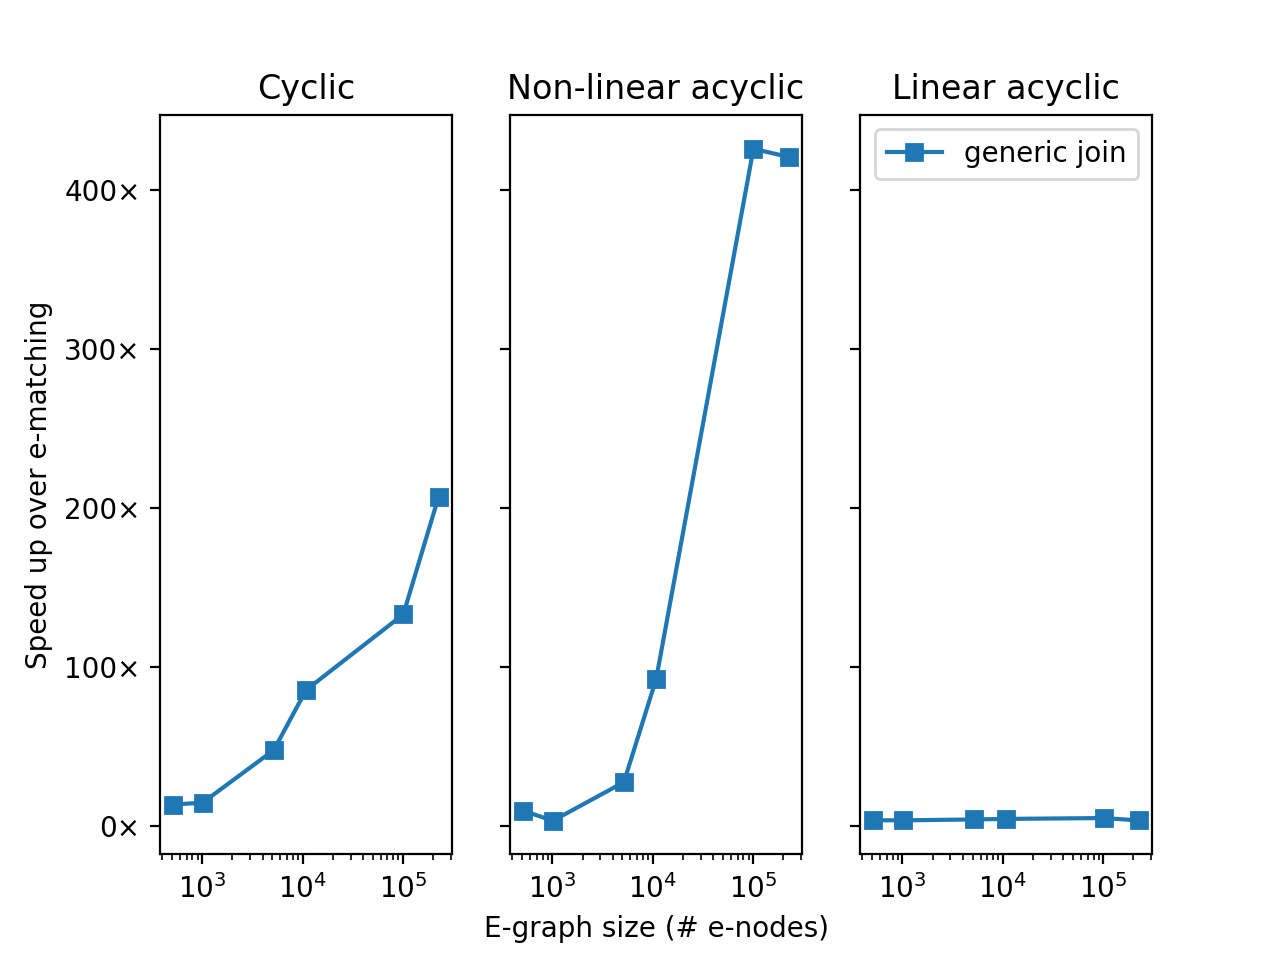
\includegraphics[width=\linewidth]{figures/egdb.png}
    \caption{Speedup of relational \ematching over backtracking-based \ematching algorithms}
    \label{fig:bench1}
\end{figure}

The result is shown in Figure \ref{fig:bench1}. On both cyclic and non-linear acyclic case, our relational \ematching achieves asymptotically better performance, up to 426$\times$, over backtracking-based \ematching by taking advantages of the equality constraints. In the linear
case, because no variable occurs more than once, relational \ematching
achieves similar performance as the backtracking-based \ematching up to a constant factor.\footnote{Note that the comparison here is between the handwritten relational \ematching, which is compiled, and the \ematching engine in \egg, which is interpreted, because this experiment is performed for the PLDI SRC, when we have not developed a fully working version of relational \ematching inside \egg. Therefore, the comparison is not perfectly apple-to-apple. However, we can still see the asymptotic trends.}

\begin{figure}
\vspace{-4em}
     \centering
     \begin{subfigure}[b]{0.8\textwidth}
         \centering
         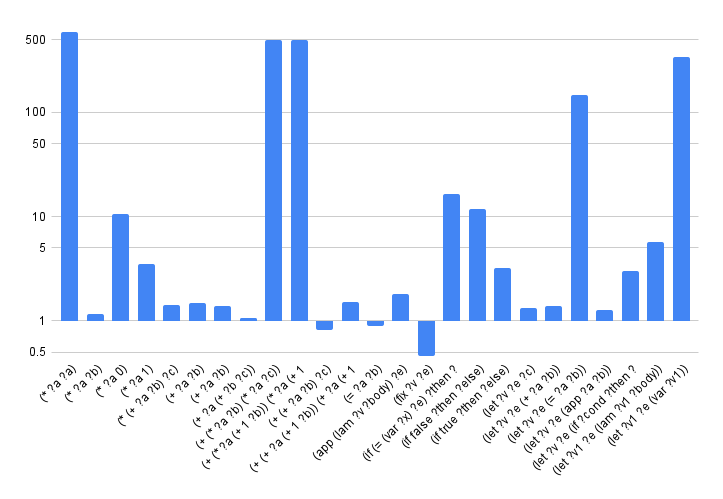
\includegraphics[width=\textwidth]{figures/bench2-1.png}
         \caption{}
         \label{bench2-1}
     \end{subfigure}
     \\
     \begin{subfigure}[b]{0.8\textwidth}
         \centering
         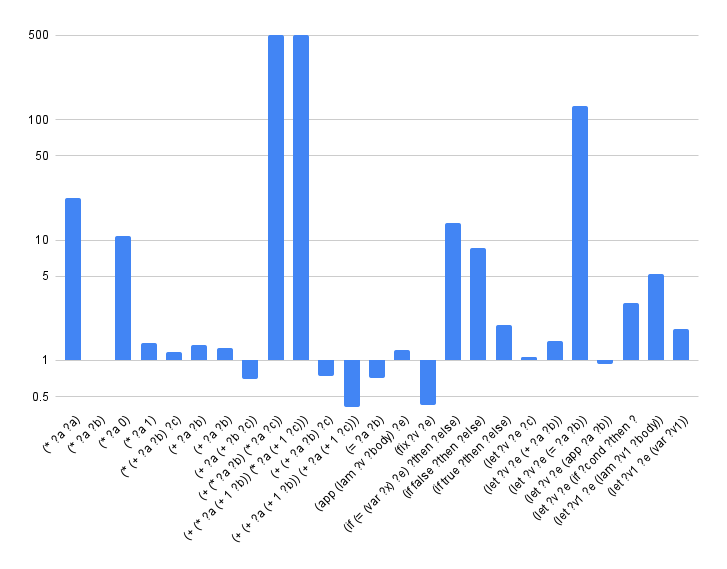
\includegraphics[width=\textwidth]{figures/bench2-0.png}
         \caption{}
         \label{bench2-0}
     \end{subfigure}
     \caption{(a) Speedup of relationl \ematching over backtracking-based \ematching on microbenchmarks without index building time. (b) Speedup of relationl \ematching over backtracking-based \ematching on microbenchmarks with index building time.}
     \label{bench2}
\end{figure}


Next, we compare the performance of relational \ematching as we implemented in \egg against \egg's original \ematching implementation on several benchmarks. The result is presented with two figures in Figure \ref{bench2}. Figure~\ref{bench2-1} only compares the enumeration procedure of backtracking-based \ematching to that of relational \ematching, excluding time that may need to build the index before performing generic join, which are shared among different patterns, and Figure~\ref{bench2-1} makes the same comparison but includes the index building time.

According to Figure~\ref{bench2-1}, relational \ematching achieves substantial speedups for complex patterns. However, on some simple patterns, relational \ematching does not achieve a significant speedup compared to backtracking-based \ematching algorithms, and sometimes relational \ematching is slower.
Most of such patterns are linear patterns like \texttt{(+ (+ ?a ?b) ?c)} and \texttt{(fix ?v ?e)}. In particular, patterns like \texttt{(fix ?v ?e)} are equivalent to a simple enumeration of all $f$-application terms for some function symbol $f$, which we call singleton patterns. The relational \ematching has the most slowdown on several singleton patterns because running singleton patterns is very fast, taking only a few microseconds, so the overhead related to relational \ematching such as query compilation dominates the run time. Still, because they only take a few microseconds, the run time for matching such patterns are not an issue for real applications. Moreover,  note the relational \ematching performs order of magnitude  better on pattern \texttt{(* ?a ?a)}, which is a singleton pattern, as our query optimizer exploits the fact that both children of the *-application node are the same and thus only does a filter over the corresponding relation. In contrast, backtracking-based \ematching without ad hoc handling can only express this as a backtracking process, which has a larger overhead.

Comparing Figure~\ref{bench2-1} against  Figure~\ref{bench2-0}, we observe the time taken for building indices to be significant. Many plans where relational \ematching is faster now becomes slower. This is consistent with the observation made by \cite{eval-wcoj}, where index building is sometimes the bottleneck of the generic join algorithm. Since our current implementation is only a prototype, we are currently working on improving the index building time so that the performance of relational \ematching is able to dominate that of the current implemented \ematching in \egg.
 
Finally, our next step of experiment is to evaluate relational \ematching on full-system applications that use \egg. We attempted to run Herbie with relational \ematching as the \ematching procedure. However, we are unable to observe any significant speedup by using relational \ematching. We speculate the cause is that the workload of Herbie is running only simple, linear patterns on small \egraphs, so there are no additional equality constraints that relational \ematching could exploit. We are working on evaluating relational \ematching on other applications, such as Tensat \citep{tensat} and Szalinski \citep{2020-pldi-szalinski-cad-eqsat}.